\documentclass{beamer}
\usetheme{metropolis}
\usepackage{graphicx}
\usepackage{booktabs}
\usepackage{tikz}
\usetikzlibrary{shapes.geometric,shapes.multipart,arrows.meta,positioning}

\title{EchoNet -- Digital Library}
\author{Team Members: \textbf{Anurag Tripathi (25M0770)}, \textbf{Viraj Ashar (25M0756)}}
\date{\today}

\begin{document}

\begin{frame}
  \titlepage
\end{frame}

\begin{frame}{Problem Statement}
  Provide a unified digital library where users can:
  \begin{itemize}
    \item Browse multiple media types (books, audiobooks, images, movies, audio, software).
    \item Use ECHODOST chatbot for quick help/Q\&A.
    \item View trending items (click-based) and featured audiobooks with read-aloud.
    \item Manage profiles and submit feedback with email acknowledgements.
  \end{itemize}
\end{frame}

\begin{frame}{Scope and Limitations}
  \begin{itemize}
    \item Scope: Multi-media browsing, featured audiobooks, trending, auth/profile, ECHODOST, feedback with DB+email, read-aloud via Web Speech API.
    \item Limitations: small curated dataset, no robust full-text search, no offline bundles, minimal moderation/admin tools.
  \end{itemize}
\end{frame}

\begin{frame}{Architecture (Data Flow)}
\begin{figure}[h]
\centering
\resizebox{0.95\linewidth}{!}{%
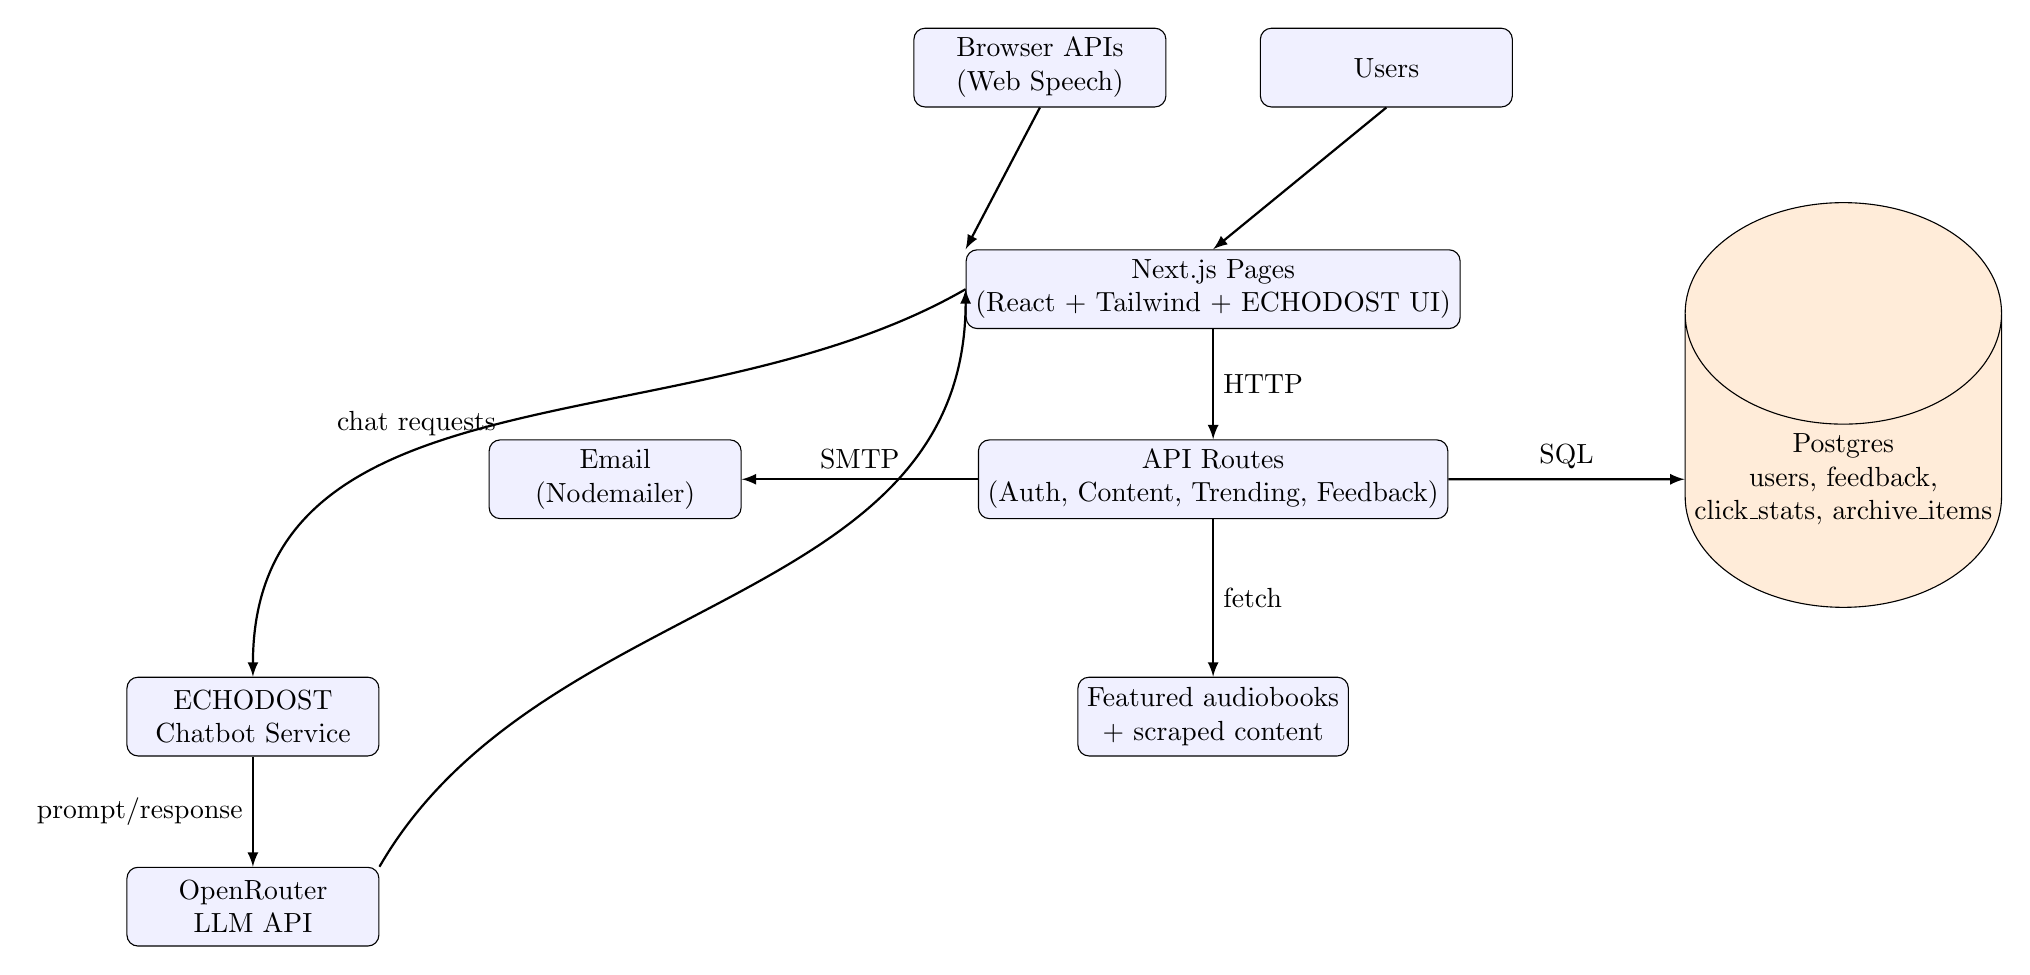
\begin{tikzpicture}[
  node distance=1.2cm and 2.4cm,
  box/.style={draw, rounded corners, align=center, minimum width=3.2cm, minimum height=1cm, fill=blue!6},
  db/.style={draw, cylinder, shape border rotate=90,
             minimum height=1.4cm, minimum width=1.1cm, aspect=0.7, align=center, fill=orange!15},
  arr/.style={-latex, thick}
]
\node[box] (ui) {Next.js Pages\\(React + Tailwind + ECHODOST UI)};
\node[box, below=1.4cm of ui] (api) {API Routes\\(Auth, Content, Trending, Feedback)};
\node[db, right=3.0cm of api] (db) {Postgres\\users, feedback,\\click\_stats, archive\_items};
\node[box, left=3.0cm of api] (mail) {Email\\(Nodemailer)};
\node[box, below=2.0cm of api] (assets) {Featured audiobooks\\+ scraped content};
\node[box, above=1.8cm of ui, xshift=-2.2cm] (browser) {Browser APIs\\(Web Speech)};
\node[box, above=1.8cm of ui, xshift=2.2cm] (users) {Users};
\node[box, below=2.0cm of mail, xshift=-4.6cm] (chat) {ECHODOST\\Chatbot Service};
\node[box, below=1.4cm of chat] (openrouter) {OpenRouter\\LLM API};

\draw[arr] (users.south) -- (ui.north);
\draw[arr] (browser.south) -- (ui.north west);
\draw[arr] (ui) -- node[right]{HTTP} (api);
\draw[arr] (api) -- node[above]{SQL} (db);
\draw[arr] (api) -- node[above]{SMTP} (mail);
\draw[arr] (api) -- node[right]{fetch} (assets);
\draw[arr] (ui.west) to[out=210,in=90] node[left]{chat requests} (chat.north);
\draw[arr] (chat.south) -- node[left]{prompt/response} (openrouter.north);
\draw[arr] (openrouter.north east) to[out=60,in=270] (ui.west);
\end{tikzpicture}%
}
\end{figure}
\end{frame}

\begin{frame}{Technologies}
  \begin{itemize}
    \item Frontend: Next.js, React, Tailwind.
    \item Backend/API: Node.js (Next API routes).
    \item Data: Postgres; static featured audiobooks list.
    \item Comms: Nodemailer (Gmail SMTP).
    \item Browser: Web Speech API (read-aloud).
    \item Chat: ECHODOST UI + OpenRouter LLM API.
  \end{itemize}
\end{frame}

\begin{frame}{Data and Audiobooks}
  \begin{itemize}
    \item 10 featured public-domain books with text (Gutenberg) and audio (LibriVox) links.
    \item Click tracking feeds trending; anchors jump into Books/audiobooks section.
    \item Advantage of scraping: after ingest, serving is independent of the Archive API.
  \end{itemize}
\end{frame}

\begin{frame}{Challenges (Observed)}
  \begin{itemize}
    \item Internet Archive limit of 10k items/request; unclear continuation beyond 10k.
    \item Large data scale: avg 8.75 MB/request; 16 requests $\approx$ 140 MB; full set $\approx$ 70.5 GB.
    \item Time: 16 requests $\approx$ 3 minutes; full scrape $\approx$ 26 hours.
    \item Slow DB-to-UI loading initially.
    \item No prior experience with chatbot.
    \item No prior experience sending emails on feedback.
  \end{itemize}
\end{frame}

\begin{frame}{Resolutions}
  \begin{itemize}
    \item Used response \texttt{cursor} to paginate beyond 10k; indexed DB to speed queries.
    \item Sampled $\sim$20k items per category to reduce complexity.
    \item Implemented Nodemailer for feedback acknowledgements.
    \item Learned chatbot implementation (ECHODOST) via documentation.
    \item Built pages with Next.js/Tailwind; used PostgreSQL for persistence.
  \end{itemize}
\end{frame}

\begin{frame}{Commit Logs — Anurag Tripathi}
  \begin{itemize}
    \item FEAT: Tweaks-2; Adding the audio book final tweaks
    \item FEAT: Contact updation and feedback
    \item FEAT: Added Profile; Removing favourite
    \item FEAT: Added Favorites page to display and manage user favorites
    \item FEAT: Implemented page design of categories (filters)
    \item FEAT: Implemented design of homepage
    \item FEAT: Created backend GET route /api/by
  \end{itemize}
\end{frame}

\begin{frame}{Commit Logs — Viraj Ashar}
  \begin{itemize}
    \item FEAT: Added logo and theme color; Implemented SVG logo
    \item FEAT: Added search bar on the homepage
    \item FEAT: Implemented chatbot using the OpenRouter gateway service
    \item FIX: Fixed designs on the homepage and category; Fixed bugs for user profile creation
    \item FEAT: Implemented trending feature
  \end{itemize}
\end{frame}

\begin{frame}{Commit Logs — Viraj Ashar}
  \begin{itemize}
    \item FEAT: Chunked the database to 1{,}000{,}000 items and fixed search filter
    \item FEAT: Created backend routes to get data on homepage and category pages
    \item FEAT: Filtered languages, subjects, years from items and inserted in DB
    \item FEAT: Script to create database from scraped JSON data
    \item FEAT: Implemented the python script to scrape archive items
    \item Setup Done
  \end{itemize}
\end{frame}

\begin{frame}{Project Screenshots — Home}
  \centering
  \includegraphics[width=\linewidth]{home.png}
\end{frame}

\begin{frame}{Project Screenshots — Movies}
  \centering
  \includegraphics[width=\linewidth]{movies.png}
\end{frame}

\begin{frame}{Project Screenshots — Images}
  \centering
  \includegraphics[width=\linewidth]{images.png}
\end{frame}

\begin{frame}{Project Screenshots — Books / Audiobooks}
  \centering
  \includegraphics[width=\linewidth]{books.png}
\end{frame}

\begin{frame}{Project Screenshots — Audio}
  \centering
  \includegraphics[width=\linewidth]{audio.png}
\end{frame}

\begin{frame}{Project Screenshots — Software}
  \centering
  \includegraphics[width=\linewidth]{software.png}
\end{frame}

\begin{frame}{Project Screenshots — Contact / Feedback}
  \centering
  \includegraphics[width=\linewidth]{contact.png}
\end{frame}

\begin{frame}{Project Screenshots — SignIn}
  \centering
  \includegraphics[width=\linewidth]{signin.png}
\end{frame}

\begin{frame}{Project Screenshots — SignUp}
  \centering
  \includegraphics[width=\linewidth]{signup.png}
\end{frame}

\begin{frame}{Project Screenshots — Profile}
  \centering
  \includegraphics[width=\linewidth]{profile.png}
\end{frame}

\begin{frame}{Future Work}
  \begin{itemize}
    \item Richer datasets.
    \item Admin dashboard for feedback and trending moderation.
    \item Offline bundles.
    \item Deeper chatbot knowledge base and analytics.
    \item Implement audio feature in ECHODOST.
  \end{itemize}
\end{frame}

\begin{frame}{Thank You}
  \begin{center}
    echo "bye, see you again..."
  \end{center}
\end{frame}

\end{document}
